\begin{figure}[!htbp]
    \centering
    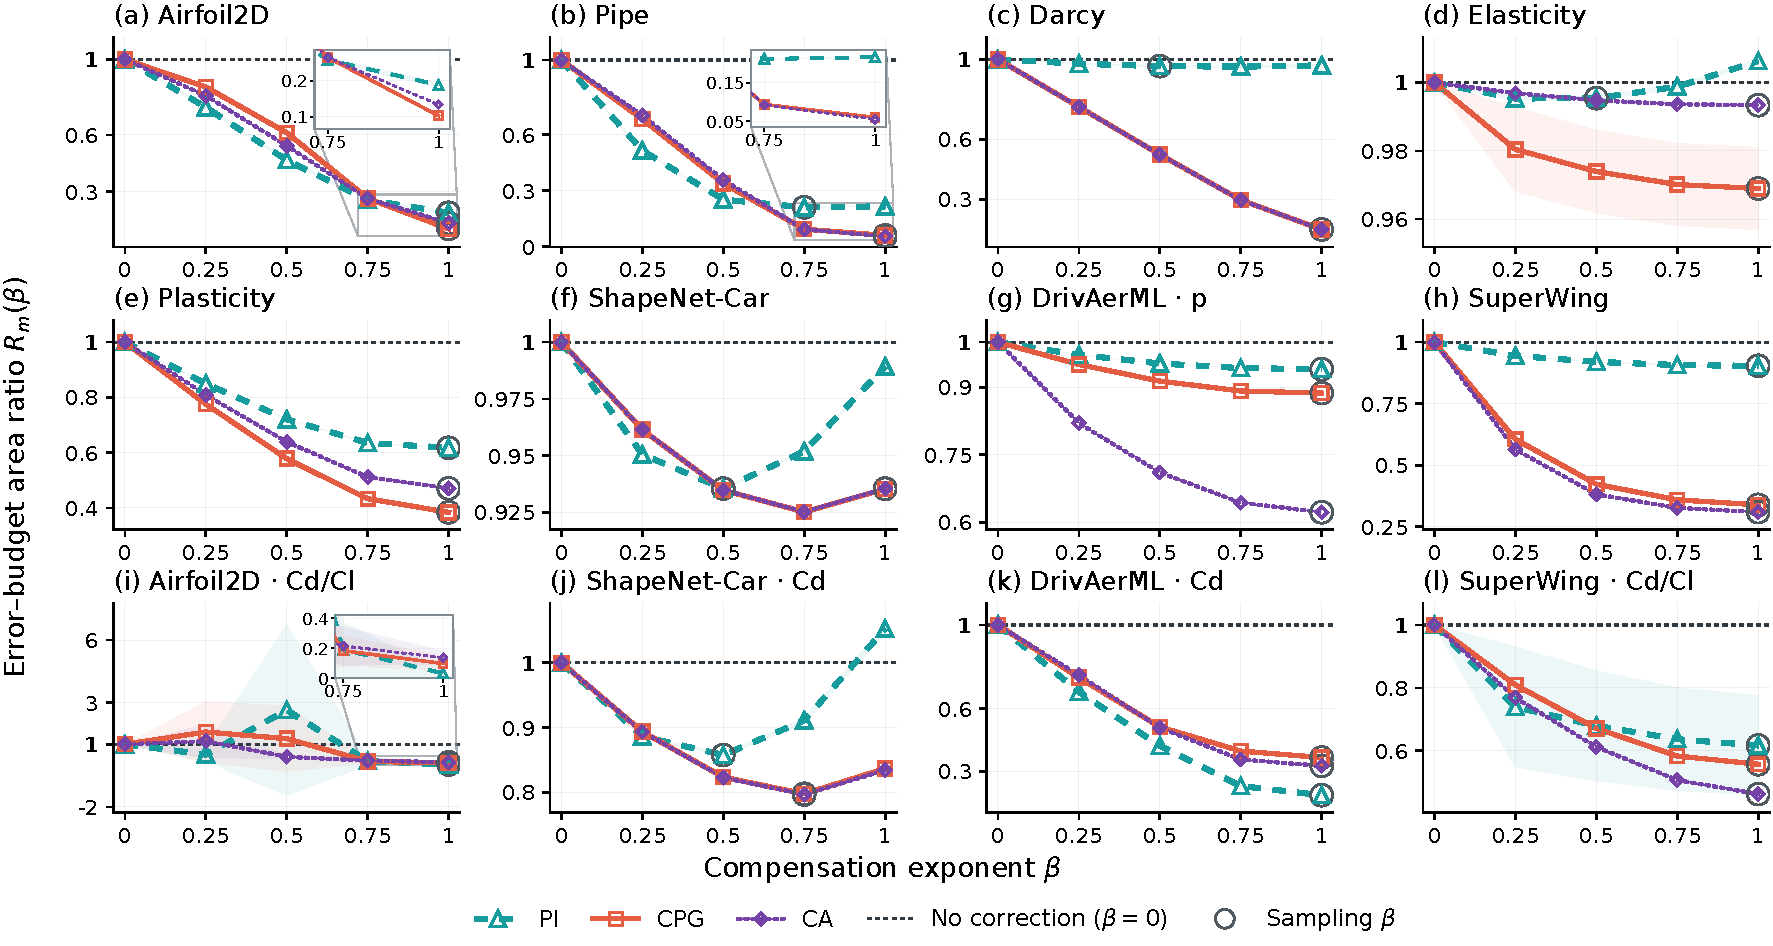
\includegraphics[width=\linewidth]{figures/appendix/beta_ablation.pdf}
\caption{\textbf{Ablation of the measure-correction exponent.}
Checkpoints, sampled points, and reconstruction are fixed. The y-axis is
$R_m(\beta)$ from \eqref{eq:beta_relative_area}: each policy and seed is
normalized to its own $\beta=0$ error--budget area before averaging.
Areas cover $37.5\%$, $50\%$, and $75\%$ budgets. Bands show one sample
standard deviation across three seeds. Gray rings (Sampling $\beta$) mark the
compensation exponent used by each policy in the main experiments.
The dashed line denotes no correction. Insets enlarge high-$\beta$
portions; the Airfoil ratio panel retains the full uncertainty envelope.
Table~\ref{tab:beta_ablation} uses Uniform-normalized rAUEC.}
\label{fig:beta_ablation}
\end{figure}
